\section{Minimal Closure and Triangular Geometry}
\label{sec:triangular}

\subsection{Reformulating the Question}

Section~\ref{sec:closure_energy} introduced closure as the condition
for structural persistence, and identified three-node configurations
as the first candidates for such structures.
The central question is:
\begin{equation}
  \boxed{\text{Why is the minimal closure unit triangular?}}
\end{equation}
This is not a geometric assumption, but a structural requirement
that must follow from the properties of closure itself.

\subsection{Two-Node Systems: Absence of Closure}

A system of two nodes permits only a bidirectional relation $i \leftrightarrow j$.
Such a system defines a connection, but not an enclosure:
no loop is formed, no area is defined, and no internal reference is possible.
Accordingly, $\Phi = 0$.
\begin{equation}
  \boxed{\text{A two-node system cannot form a self-sustaining structure.}}
\end{equation}

\subsection{Three-Node Systems: Emergence of Closure}

With three nodes $(i,j,k)$, a closed loop $i \to j \to k \to i$ becomes possible.
This configuration introduces a minimal loop, a definable area,
and mutual reference among nodes.
The closure condition is:
\begin{equation}
  \vec{e}_i + \vec{e}_j + \vec{e}_k \approx 0,
\end{equation}
which simultaneously encodes vector balance, structural consistency,
and enclosure stability.
\begin{equation}
  \boxed{\text{Three nodes form the minimal self-referential enclosure.}}
\end{equation}

\subsection{Higher-Node Systems: Decomposition into Triangles}

For $n \geq 4$, closure structures can always be decomposed into
triangular components:
\begin{equation}
  \text{closure}(n) \;\longrightarrow\; \sum \text{triangular closures}.
\end{equation}
No fundamentally new minimal unit appears beyond three nodes.
\begin{equation}
  \boxed{\text{Triangles are the irreducible units of closure geometry.}}
\end{equation}

\subsection{Uniqueness of the Triangle}

\begin{center}
\begin{tabular}{ll}
\toprule
Node count & Structural property \\
\midrule
2   & No closure \\
3   & Minimal closure \\
4+  & Composite of triangles \\
\bottomrule
\end{tabular}
\end{center}
\begin{equation}
  \boxed{\text{The triangle is the unique minimal closure unit.}}
\end{equation}
This uniqueness follows from the minimal conditions required
for internal consistency and self-reference,
not from geometric convenience.

\subsection{Modes of Triangular Closure}

Not all triangular closures are equivalent.
Three structural regimes can be identified:
\begin{enumerate}
  \item \textbf{Non-degenerate triangle} ---
        finite area, three independent directions, maximal structural stability.
  \item \textbf{Degenerate triangle} ---
        area approaches zero, reduced dimensionality,
        constrained degrees of freedom.
  \item \textbf{Extreme degeneracy} ---
        collapse of area, effectively point-like, minimal internal structure.
\end{enumerate}
\begin{equation}
  \boxed{\text{Structural behavior depends on the degree of triangular degeneracy.}}
\end{equation}

These three regimes are summarized in Fig.~\ref{fig:closure_triangle}.

\begin{figure}[h]
  \centering
  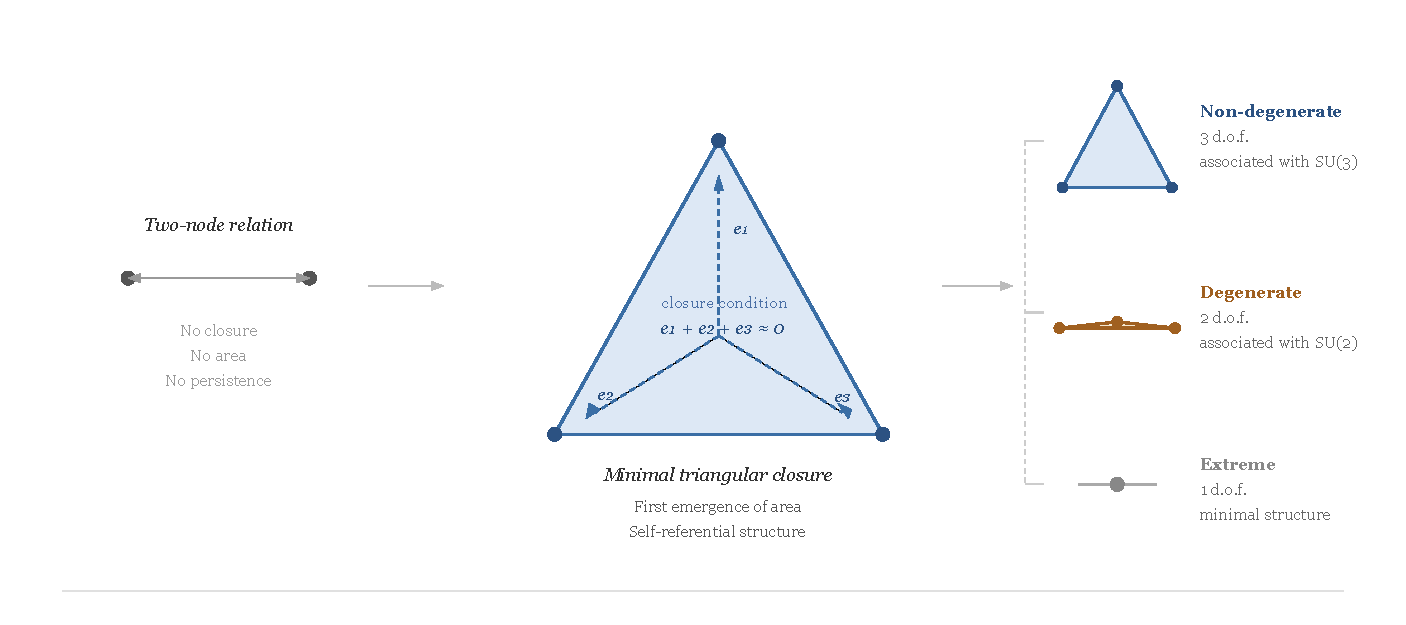
\includegraphics[width=\textwidth]{figures/VED_Vol2_Figure1.pdf}
  \caption{
    Closure does not occur in two-node systems, where no loop or area is defined.
    The triangle is the minimal configuration supporting closure,
    where vector balance and enclosed area first emerge.
    Triangular closure admits three structural regimes depending on degeneracy:
    non-degenerate (full area), degenerate (collapsed area), and extreme degeneracy.
    These regimes correspond to different structural degrees of freedom,
    which are associated with distinct symmetry structures in subsequent analysis.
  }
  \label{fig:closure_triangle}
\end{figure}

\subsection{Toward Symmetry}

The triangle is established as the minimal closure unit,
but it also carries internal degrees of freedom.
The next step is to understand which transformations leave closure invariant.
This leads directly to the emergence of gauge symmetry in the following section.
